\documentclass[12pt]{article}
\setlength\parindent{0pt}
\usepackage[margin=1in]{geometry} 
\usepackage{amsmath,amsthm,amssymb,amsfonts}  
\usepackage[utf8]{inputenc}
\usepackage{xpatch} 
\usepackage{bm}
\usepackage{cancel}
\usepackage{tikz}
\usepackage{graphicx}
\usepackage{changepage}
\usepackage{listings}
\usepackage[margin=1in]{geometry}
\usepackage{fancyhdr}
\pagestyle{fancy}
\usepackage{amsmath}
\usepackage{amssymb}
\usepackage[utf8]{inputenc}


\lhead{R2 H18 Løsningsforslag}
\rhead{Med minimal forklaring og forbehold om feil}
\begin{document}
	\begin{flushleft}
		\section{Del 1}
		\subsection{Oppgave 1}
		\textbf{a)} $$f'(x)=6(-\sin(2x-1)) \cdot \frac{\text{d}}{\text{d}x}\left[2x-1\right]=-12\sin(2x-1)$$ 
		\textbf{b)} $$g'(x)=\frac{\text{d}}{\text{d}x}\left[\cos^2(x)+\sin^2(x) \right] = \frac{\text{d}}{\text{d}x}[1] = 0$$
		
		\subsection{Oppgave 2}
		\textbf{a)} $$ \int \left(2x^2-3x\right) \, \text{d}x = \frac23 x^3 - \frac32 x^2 + C$$ 
		\textbf{b)} La $u=x^2+2 \implies \text{d}x = \frac{1}{2x} \, \text{d}u$. Da fås $$\int 4x \cdot \cos(x^2+2) \, \text{d}x = 2\int \cos(u) = 2\sin(u) + C = 2\sin(x^2+2) + C$$
		\textbf{c)} Observer at $x^2-4=(x+2)(x-2)$ og bruk delbrøksoppspalting. Det gir $$\int \frac{4}{x^2-4} = \int \left(\frac{1}{x-2} - \frac{1}{x+2} \right) \, \text{d}x = \ln|x-2| - \ln|x+2| + C = \ln \left| \frac{x-2}{x+2}\right| + C$$
		
		\subsection{Oppgave 3}
		\textbf{a)} For at rekka skal konvergere må $|e^{-x}| < 1$. Siden $e^x>0$ for alle $x \in \mathbb{R}$, holder det med å sjekke når $e^{-x} < 1 \Longleftrightarrow e^x>1 \Longleftrightarrow x > 0$ \newline
		\textbf{b)} Vi ønsker å løse $S(x)=3$. Siden $S(x)$ er en geometrisk rekke er den for alle $x>0$ slik at $$S(x)=\frac{1}{1-e^{-x}}=\frac{e^x}{e^x-1}$$ Sett nå dette lik $3$ så får vi likningen $$ 2e^x=3 \Longleftrightarrow x = \ln\left(\frac32\right)$$
		
		\subsection{Oppgave 4}
		\textbf{b)} Vi skal finne skjæringspunktene til $\sin(x)$ og $\cos(x)$, altså løse $\sin(x)-\cos(x)=0 \Longleftrightarrow \frac{\sin(x)}{\cos(x)} - 1 = 0$, når $\cos(x)\neq 0$. Dette forenkles igjen til $\tan(x)=1$, som skjer når $x=\frac{\pi}{4} + \pi n$, $n \in \mathbb{Z}$. Så skjæringspunktene er $(\frac{\pi}{4}, \frac{\sqrt{2}}{2})$ og $(\frac{5\pi}{4}, -\frac{\sqrt{2}}{{2}})$. \newline
		
		\textbf{c)} $$\int_{\pi/4}^{5\pi/4} \left(\sin(x) - \cos(x)\right) \, \text{d}x = -\cos(x)-\sin(x)\bigg\vert_{\pi/4}^{5\pi/4} = 2\sqrt{2}$$
		
		\subsection{Oppgave 5}
		\textbf{a)}Vi observerer at amplituden er $1.2$ og at perioden er $8$ sekunder. Jeg tolker likevektslinja til å være $1.2 \, \text{m}$ utifra oppgavebeskrivelsen. Siden $f(t)$ er på sitt høyeste når $t=0$, kan vi konkludere med at den er faseforskjøvet med $\frac{\pi}{2}$. Konklusjonen er $$f(t)=1.2\sin\left(\frac{\pi}{4}t + \frac{\pi}{2} \right) + 1.2$$
		\textbf{b)} Her skal vi løse $f(t)=1.2+0.6=1.8 \Longleftrightarrow \sin\left(\frac\pi4 t + \frac\pi2 \right)=\frac12$. Dette er ekvivalent med å løse $$\frac\pi4 t + \frac\pi2 = \frac\pi6 + 2\pi n \qquad \text{ og } \qquad \frac\pi4 t + \frac\pi2 = \frac{5\pi}{6} + 2\pi n$$ der $n \in \mathbb{Z}$ og $t \in [0,8]$. Dette er igjen ekvivalent med å løse $$t=-\frac{4}{3} + 8n \qquad \text{og} \qquad t=\frac43 + 8n$$ Herifra ser vi at løsningene på det ønskede intervallet er $t\in\{\frac43, \frac{20}{3}\}$ Så bøyen er 0.6m over likevektslinja etter $1.33$ sekunder og etter $6.66$ sekunder.
		
		\subsection{Oppgave 6}
		\textbf{a)} Observer at tangenten i $(1,-1)$ peker nedover, så alternativ $1$ ($y'=x+y$) kan ikke være rett, fordi da hadde $y'=1-1=0$ i $(1,-1)$, altså skulle tangenten vært flat. Hvis alternativ $2$ hadde vært korrekt skulle tangenten gått mot å stige mer og mer når $y$ nærmet seg $0$ og $x$ er liten (og positiv i dette eksempelet), for når $y'=\frac{x}{y}$, og $y\to 0$, vokser helt klart $y'$. Men her går $y'$ mot å være mer og mer "flat". Eneste gjenstående alternativ er alternativ 3, så $y'=x\cdot y$ må være korrekt. \newline
		
		\textbf{b)} $y'=x\cdot y \Longleftrightarrow \frac{y'}{y} = x$ Dette er en seperabel diff.likning., vi får $$\int \frac{1}{y} \, \text{d}y = \int x \, \text{d}x \Longleftrightarrow \ln|y| = \frac{1}{2}x^2 + C \Longleftrightarrow y = Ce^{\frac12 x^2}$$
		
		\subsection{Oppgave 7}
		\textbf{a)} $\overrightarrow{AB} = (2,-2,-1)$, $\overrightarrow{AC}=(0,-1,1)$ \newline
		
		\textbf{b)} $A(-1,1,1)$ inn i planlikningen gir $3(-1) + 2(1) + 2(1) - 1=-3+2+2-1=0$ så $A$ ligger i planet. Akkurat den samme prosessen kan brukes for å vise at $B$ og $C$ ligger i planet. \newline
		
		\textbf{c)} Vi er gitt $D(s^2-1,3s+1,10)$, $s \in \mathbb{R}$. Vektorene $\overrightarrow{AB}$, $\overrightarrow{AC}$ og $\overrightarrow{AD}$ utspenner et tetraeder $ABCD$ med volum $$V=\frac16 \left | (\overrightarrow{AB} \times \overrightarrow{AC}) \cdot \overrightarrow{AD}\right |$$ Vi regner ut at $\overrightarrow{AD}=(s^2,3s,9)$ ,og at $\overrightarrow{AB} \times \overrightarrow{AC} = (-3,-2,-2)$, så vi får at $$V=\frac16 \left| (-3,-2,-2) \cdot (s^2,3s,9) \right|=\frac{1}{6}\left|-3s^2-6s-18 \right|=\frac{1}{6}|-3||s^2+2s+6|=\frac12 |s^2+2s+6|$$ Observer at $s^2+2s+6=(s+1)^2+5$, så $s^2+2s+6$ er aldri negativ, og vi kan se bort ifra absoluttverditegnet, så funksjonen for volumet av s er gitt ved$$V(s)=\frac12s^2+s+3$$
		
		\textbf{d)} Deriverer vi $V(s)$, får vi at $V'(s)=s+1$ så $V'(s)=0$ når $s=-1$. Observer at $V'(-2)=-1$ og $V'(0)=1$, så $(-1,V(-1))$ er et bunnpunkt. Det minste volumet tetraederet kan ha er altså $V(-1)=\frac12 -1 + 3 = \frac52$.
		
		\subsection{Oppgave 8}
		Vi skal vise at $P(n): \enspace1^3+2^3+\dots+n^3=\frac{n^2(n+1)^2}{4}$ ved induksjon. \newline
		
		\textbf{Basistilfellet}, $n=1$ gir venstre side lik $1^3=1$ og høyre side $\frac{1^2(1+1)^2}{4}=1$, så høyre side er lik venstre side og basistilfellet stemmer. \newline
		
		\textbf{Induksjonshypotesen}, $n=k$. Vi antar at formelen stemmer for $n=k$, altså at $$1^3+2^3+\dots+k^3 = \frac{k^2(k+1)^2}{4}$$ 
		
		\textbf{Induksjonssteget}, vi ønsker nå å vise at $P(k)\implies P(k+1)$. 
		\begin{alignat*}{2}
			1^3+2^3+\dots+k^3+(k+1)^3 &\overset{\text{i.h}}{=} \frac{k^2(k+1)^2}{4} + (k+1)^3 \\
			&= (k+1)^2\left(\frac{k^2}{4} + (k+1)\right) \\
			&= (k+1)^2 \left(\frac{k^2+4k+4}{4}\right) \\
			&= (k+1)^2 \left(\frac{(k+2)^2}{4}\right) \\
			&= \frac{(k+1)^2((k+1)+1)^2}{4}
		\end{alignat*}
		\newpage
		\section{Del 2}
		\subsection{Oppgave 1}
		\textbf{b)} Fra oppgave a) vet man allerede hvordan dette området ser ut. Skjæringspunktene fås ved å løse $f(x)=g(x)$. Vi får at skjæringspunktene er $\{0,2\}$. Da er $$M=\int_0^2 (g(x)-f(x)) \, \text{d}x = \int_0^2 (-x^4+4x^3-6x^2+4x) \, \text{d}x = \frac85$$
		
		\textbf{c)} \\
		\begin{figure}[ht]
			\centering
			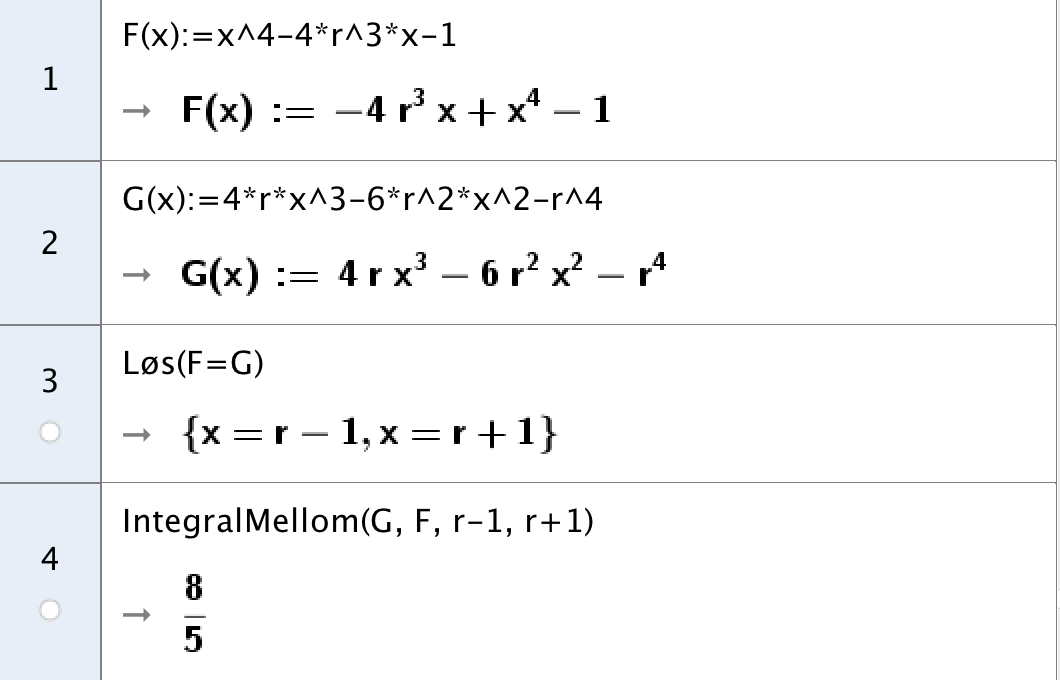
\includegraphics[width=0.7\linewidth]{ggb1.png}
		\end{figure}
		Vi ser at arealet mellom grafen er uavhengig av $r$.
		
		\subsection{Oppgave 2}
		\textbf{a)} Sentrumet i kuleflaten $K_1$ er gitt ved $(2t,1,3)$ og kulen har radius $2$. Formelen for en kuleflate med radius $r$ og sentrum i $(x_0,y_0,z_0)$ er gitt ved $(x-x_0)^2+(y-y_0)^2+(z-z_0)^2=r^2$. Så for vår del blir likningen $$(x-2t)^2+(y-1)^2+(z-3)^2=2^2$$ 
		
		\textbf{b)} $K_1$ vil tangere $yz$-planet når avstanden fra sentrum i $K_1$ til $yz$-planet er $2$. $yz$-planet har likningen $x=0$ Bruker vi nå avstandsformelen får vi at avstanden er $$D=\frac{|ax_1+d|}{\sqrt{a^2}} = \frac{1\cdot2t}{\sqrt{1^2}}=2t$$ Så vi må løse $2t=2$, altså tangerer $K_1$ $yz$-planet når $t=1$. \newline
		
		\textbf{c)} Vi har en ny kuleflate gitt ved $K_2:\, x^2+y^2+z^2=r^2$. Herifra er det lett å se at sentrum for $K_2$ er $(0,0,0)$. Dersom $r=2$, vil kulene tangere hverandre når avstanden mellom sentrumene til $K_1$ og $K_2$ er $4$ (radius $K_1$ + radius $K_2$). Altså må vi finne når avstanden mellom $(0,0,0)$ og $(2t,1,3)$ er $4$. Avstanden mellom disse punktene er $S=\sqrt{(2t)^2+1^2+3^2}=\sqrt{4t^2+10}$. Løser vi $\sqrt{4t^2+10}=4$, får vi $t^2=\frac32$, så $t=\pm \sqrt{\frac32}$ Altså vil kulene tangere hverandre når $t=\displaystyle \left \{-\sqrt{\frac{3}{2}}, \sqrt{\frac32}\right \}$. \newline
		
		\textbf{d)} Fra c) vet vi at avstanden mellom sentrumene, hvis $K_2$ har radius $r$, er $A(t)=\sqrt{4t^2+10}$, og at kulene tangerer hverandre når $A(t)=2+r$. Setter vi $A(t)=2+r$, får vi likningen $4t^2+10=4+4r+r^2 \Longleftrightarrow t^2 = \frac14r^2+r-\frac{3}{2}$. Siden $t^2\geq0$ for alle $t \in \mathbb{R}$, må vi ha at $\frac14r^2+r-\frac{3}{2}\geq0$. Denne likningen har to løsninger, der henholdsvis en er positiv, nemlig $r=\sqrt{10}-2$. Altså er $r=\sqrt{10}-2$ den minste verdien som sørger for at de to kulene tangerer.
		
		\subsection{Oppgave 3}
		\textbf{a)} Hvis bedriften klarer å nå målet blir utslippet i 2018 lik 20 000 tonn, i 2019 lik $20 000\cdot(0.85)$, i 2020 vil den være $(20000\cdot 0.85)\cdot 0.85 = 20000 \cdot 0.85^2$. Vi ser at mønsteret danner en geometrisk rekke, så fra 2018 til 2027 blir summen av utslippene lik $$\sum_{n=0}^9 20000\cdot 0.85^n \approx 107083.4 \, \text{ (tonn)}$$
		
		\textbf{b)} Om en annen bedrift vet vi at utslippene deres over $2018-2027$ er $$S(r)\sum_{n=0}^{9} 30000\cdot r^n$$ Vi er bedt å finne $r$ slik at bedriften i a) og denne bedriften slipper ut like mye. Formelen for summen av en geometrisk rekke lar oss omskrive $S(r)$ til $$S(r)=30000 \left(\frac{1-r^9}{1-r}\right)$$ Settes $S(r)$ lik svaret i a) (dette kan man for eksempel gjøre i CAS), fås $r\approx 0.74$, så bedriften må redusere utslippene hvert år med omtrent $74 \%$ for at bedriftene skal slippe ut det samme over samme periode.
		
		\subsection{Oppgave 4}
		\textbf{a)} $3.2$ sier oss at det renner inn $3.2$ liter vann i tanken per min, $0.14$ sier oss at det renner ut $14\%$ av innholdet i tanken per minutt og $y(0)=200$ sier oss at det var $200$ liter vann i tanken til å starte med. \newline
		
		\textbf{b)} Dette er en lineær første ordens diff.likning $$y'+0.14y=3.2$$ Integrerende faktor er $e^{\int 0.14 \, \text{d}x} = e^{0.14x}$ Vi får 
		\begin{alignat*}{2}
			e^{0.14x}\left(y'+0.14y\right) &= 3.2e^{0.14x} \\
			\left(ye^{0.14x} \right)' &= 3.2e^{0.14x} \\
			\int \left(ye^{0.14x} \right)' \, \text{d}x &= \int 3.2e^{0.14x} \, \text{d}x \\
			ye^{0.14x} &= \frac{160}{7}e^{0.14x} + C \\
			y &= \frac{160}{7} + Ce^{-0.14x}
		\end{alignat*}
		Med initialverdibetingelsen $y(0)=200$ fås $C=200-\frac{160}{7} = \frac{1240}{7}$, så $$y=\frac{160}{7} + \frac{1240}{7}e^{-0.14x}$$
		
		\textbf{c)} $y(20) \approx 33.63 \enspace \text{(liter)}$ \newline
		
		\textbf{d)} Utifra opplysningene danner vi oss diff.likningen $y'=1.5-ky$ for en $k \in \mathbb{R}$, der $y(0)=0$. Denne diff.likningen kan løses likt som i b) og vi får den generelle løsningen $$y=\frac{1.5}{k} + Ce^{-kx}$$ Med initialverdibetingelsen $y(0)=0$ fås $$y=\frac{1.5}{k} - \frac{1.5}{k}e^{-kx}$$ Videre vet vi at mengden vann i tanken vil stabilisere seg på 10L etterhvert, med andre ord er $$\lim_{x \to \infty} \left[\frac{1.5}{k} - \frac{1.5}{k}e^{-kx}\right] = 10$$ Vi kan herifra konkludere at $k=\dfrac{1.5}{10}$ Så funksjonen vår er gitt ved $$y=10-10e^{-0.15x}$$ Og etter 20 minutter vil da derfor være $$y(20)\approx 9.50 \enspace (\text{liter i tanken})$$
		\end{flushleft}
	
\end{document}
